% Options for packages loaded elsewhere
% Options for packages loaded elsewhere
\PassOptionsToPackage{unicode}{hyperref}
\PassOptionsToPackage{hyphens}{url}
\PassOptionsToPackage{dvipsnames,svgnames,x11names}{xcolor}
%
\documentclass[
  letterpaper,
  DIV=11,
  numbers=noendperiod]{scrreprt}
\usepackage{xcolor}
\usepackage{amsmath,amssymb}
\setcounter{secnumdepth}{5}
\usepackage{iftex}
\ifPDFTeX
  \usepackage[T1]{fontenc}
  \usepackage[utf8]{inputenc}
  \usepackage{textcomp} % provide euro and other symbols
\else % if luatex or xetex
  \usepackage{unicode-math} % this also loads fontspec
  \defaultfontfeatures{Scale=MatchLowercase}
  \defaultfontfeatures[\rmfamily]{Ligatures=TeX,Scale=1}
\fi
\usepackage{lmodern}
\ifPDFTeX\else
  % xetex/luatex font selection
\fi
% Use upquote if available, for straight quotes in verbatim environments
\IfFileExists{upquote.sty}{\usepackage{upquote}}{}
\IfFileExists{microtype.sty}{% use microtype if available
  \usepackage[]{microtype}
  \UseMicrotypeSet[protrusion]{basicmath} % disable protrusion for tt fonts
}{}
\makeatletter
\@ifundefined{KOMAClassName}{% if non-KOMA class
  \IfFileExists{parskip.sty}{%
    \usepackage{parskip}
  }{% else
    \setlength{\parindent}{0pt}
    \setlength{\parskip}{6pt plus 2pt minus 1pt}}
}{% if KOMA class
  \KOMAoptions{parskip=half}}
\makeatother
% Make \paragraph and \subparagraph free-standing
\makeatletter
\ifx\paragraph\undefined\else
  \let\oldparagraph\paragraph
  \renewcommand{\paragraph}{
    \@ifstar
      \xxxParagraphStar
      \xxxParagraphNoStar
  }
  \newcommand{\xxxParagraphStar}[1]{\oldparagraph*{#1}\mbox{}}
  \newcommand{\xxxParagraphNoStar}[1]{\oldparagraph{#1}\mbox{}}
\fi
\ifx\subparagraph\undefined\else
  \let\oldsubparagraph\subparagraph
  \renewcommand{\subparagraph}{
    \@ifstar
      \xxxSubParagraphStar
      \xxxSubParagraphNoStar
  }
  \newcommand{\xxxSubParagraphStar}[1]{\oldsubparagraph*{#1}\mbox{}}
  \newcommand{\xxxSubParagraphNoStar}[1]{\oldsubparagraph{#1}\mbox{}}
\fi
\makeatother

\usepackage{color}
\usepackage{fancyvrb}
\newcommand{\VerbBar}{|}
\newcommand{\VERB}{\Verb[commandchars=\\\{\}]}
\DefineVerbatimEnvironment{Highlighting}{Verbatim}{commandchars=\\\{\}}
% Add ',fontsize=\small' for more characters per line
\usepackage{framed}
\definecolor{shadecolor}{RGB}{241,243,245}
\newenvironment{Shaded}{\begin{snugshade}}{\end{snugshade}}
\newcommand{\AlertTok}[1]{\textcolor[rgb]{0.68,0.00,0.00}{#1}}
\newcommand{\AnnotationTok}[1]{\textcolor[rgb]{0.37,0.37,0.37}{#1}}
\newcommand{\AttributeTok}[1]{\textcolor[rgb]{0.40,0.45,0.13}{#1}}
\newcommand{\BaseNTok}[1]{\textcolor[rgb]{0.68,0.00,0.00}{#1}}
\newcommand{\BuiltInTok}[1]{\textcolor[rgb]{0.00,0.23,0.31}{#1}}
\newcommand{\CharTok}[1]{\textcolor[rgb]{0.13,0.47,0.30}{#1}}
\newcommand{\CommentTok}[1]{\textcolor[rgb]{0.37,0.37,0.37}{#1}}
\newcommand{\CommentVarTok}[1]{\textcolor[rgb]{0.37,0.37,0.37}{\textit{#1}}}
\newcommand{\ConstantTok}[1]{\textcolor[rgb]{0.56,0.35,0.01}{#1}}
\newcommand{\ControlFlowTok}[1]{\textcolor[rgb]{0.00,0.23,0.31}{\textbf{#1}}}
\newcommand{\DataTypeTok}[1]{\textcolor[rgb]{0.68,0.00,0.00}{#1}}
\newcommand{\DecValTok}[1]{\textcolor[rgb]{0.68,0.00,0.00}{#1}}
\newcommand{\DocumentationTok}[1]{\textcolor[rgb]{0.37,0.37,0.37}{\textit{#1}}}
\newcommand{\ErrorTok}[1]{\textcolor[rgb]{0.68,0.00,0.00}{#1}}
\newcommand{\ExtensionTok}[1]{\textcolor[rgb]{0.00,0.23,0.31}{#1}}
\newcommand{\FloatTok}[1]{\textcolor[rgb]{0.68,0.00,0.00}{#1}}
\newcommand{\FunctionTok}[1]{\textcolor[rgb]{0.28,0.35,0.67}{#1}}
\newcommand{\ImportTok}[1]{\textcolor[rgb]{0.00,0.46,0.62}{#1}}
\newcommand{\InformationTok}[1]{\textcolor[rgb]{0.37,0.37,0.37}{#1}}
\newcommand{\KeywordTok}[1]{\textcolor[rgb]{0.00,0.23,0.31}{\textbf{#1}}}
\newcommand{\NormalTok}[1]{\textcolor[rgb]{0.00,0.23,0.31}{#1}}
\newcommand{\OperatorTok}[1]{\textcolor[rgb]{0.37,0.37,0.37}{#1}}
\newcommand{\OtherTok}[1]{\textcolor[rgb]{0.00,0.23,0.31}{#1}}
\newcommand{\PreprocessorTok}[1]{\textcolor[rgb]{0.68,0.00,0.00}{#1}}
\newcommand{\RegionMarkerTok}[1]{\textcolor[rgb]{0.00,0.23,0.31}{#1}}
\newcommand{\SpecialCharTok}[1]{\textcolor[rgb]{0.37,0.37,0.37}{#1}}
\newcommand{\SpecialStringTok}[1]{\textcolor[rgb]{0.13,0.47,0.30}{#1}}
\newcommand{\StringTok}[1]{\textcolor[rgb]{0.13,0.47,0.30}{#1}}
\newcommand{\VariableTok}[1]{\textcolor[rgb]{0.07,0.07,0.07}{#1}}
\newcommand{\VerbatimStringTok}[1]{\textcolor[rgb]{0.13,0.47,0.30}{#1}}
\newcommand{\WarningTok}[1]{\textcolor[rgb]{0.37,0.37,0.37}{\textit{#1}}}

\usepackage{longtable,booktabs,array}
\usepackage{calc} % for calculating minipage widths
% Correct order of tables after \paragraph or \subparagraph
\usepackage{etoolbox}
\makeatletter
\patchcmd\longtable{\par}{\if@noskipsec\mbox{}\fi\par}{}{}
\makeatother
% Allow footnotes in longtable head/foot
\IfFileExists{footnotehyper.sty}{\usepackage{footnotehyper}}{\usepackage{footnote}}
\makesavenoteenv{longtable}
\usepackage{graphicx}
\makeatletter
\newsavebox\pandoc@box
\newcommand*\pandocbounded[1]{% scales image to fit in text height/width
  \sbox\pandoc@box{#1}%
  \Gscale@div\@tempa{\textheight}{\dimexpr\ht\pandoc@box+\dp\pandoc@box\relax}%
  \Gscale@div\@tempb{\linewidth}{\wd\pandoc@box}%
  \ifdim\@tempb\p@<\@tempa\p@\let\@tempa\@tempb\fi% select the smaller of both
  \ifdim\@tempa\p@<\p@\scalebox{\@tempa}{\usebox\pandoc@box}%
  \else\usebox{\pandoc@box}%
  \fi%
}
% Set default figure placement to htbp
\def\fps@figure{htbp}
\makeatother


% definitions for citeproc citations
\NewDocumentCommand\citeproctext{}{}
\NewDocumentCommand\citeproc{mm}{%
  \begingroup\def\citeproctext{#2}\cite{#1}\endgroup}
\makeatletter
 % allow citations to break across lines
 \let\@cite@ofmt\@firstofone
 % avoid brackets around text for \cite:
 \def\@biblabel#1{}
 \def\@cite#1#2{{#1\if@tempswa , #2\fi}}
\makeatother
\newlength{\cslhangindent}
\setlength{\cslhangindent}{1.5em}
\newlength{\csllabelwidth}
\setlength{\csllabelwidth}{3em}
\newenvironment{CSLReferences}[2] % #1 hanging-indent, #2 entry-spacing
 {\begin{list}{}{%
  \setlength{\itemindent}{0pt}
  \setlength{\leftmargin}{0pt}
  \setlength{\parsep}{0pt}
  % turn on hanging indent if param 1 is 1
  \ifodd #1
   \setlength{\leftmargin}{\cslhangindent}
   \setlength{\itemindent}{-1\cslhangindent}
  \fi
  % set entry spacing
  \setlength{\itemsep}{#2\baselineskip}}}
 {\end{list}}
\usepackage{calc}
\newcommand{\CSLBlock}[1]{\hfill\break\parbox[t]{\linewidth}{\strut\ignorespaces#1\strut}}
\newcommand{\CSLLeftMargin}[1]{\parbox[t]{\csllabelwidth}{\strut#1\strut}}
\newcommand{\CSLRightInline}[1]{\parbox[t]{\linewidth - \csllabelwidth}{\strut#1\strut}}
\newcommand{\CSLIndent}[1]{\hspace{\cslhangindent}#1}



\setlength{\emergencystretch}{3em} % prevent overfull lines

\providecommand{\tightlist}{%
  \setlength{\itemsep}{0pt}\setlength{\parskip}{0pt}}



 


\KOMAoption{captions}{tableheading}
\makeatletter
\@ifpackageloaded{tcolorbox}{}{\usepackage[skins,breakable]{tcolorbox}}
\@ifpackageloaded{fontawesome5}{}{\usepackage{fontawesome5}}
\definecolor{quarto-callout-color}{HTML}{909090}
\definecolor{quarto-callout-note-color}{HTML}{0758E5}
\definecolor{quarto-callout-important-color}{HTML}{CC1914}
\definecolor{quarto-callout-warning-color}{HTML}{EB9113}
\definecolor{quarto-callout-tip-color}{HTML}{00A047}
\definecolor{quarto-callout-caution-color}{HTML}{FC5300}
\definecolor{quarto-callout-color-frame}{HTML}{acacac}
\definecolor{quarto-callout-note-color-frame}{HTML}{4582ec}
\definecolor{quarto-callout-important-color-frame}{HTML}{d9534f}
\definecolor{quarto-callout-warning-color-frame}{HTML}{f0ad4e}
\definecolor{quarto-callout-tip-color-frame}{HTML}{02b875}
\definecolor{quarto-callout-caution-color-frame}{HTML}{fd7e14}
\makeatother
\makeatletter
\@ifpackageloaded{bookmark}{}{\usepackage{bookmark}}
\makeatother
\makeatletter
\@ifpackageloaded{caption}{}{\usepackage{caption}}
\AtBeginDocument{%
\ifdefined\contentsname
  \renewcommand*\contentsname{Table of contents}
\else
  \newcommand\contentsname{Table of contents}
\fi
\ifdefined\listfigurename
  \renewcommand*\listfigurename{List of Figures}
\else
  \newcommand\listfigurename{List of Figures}
\fi
\ifdefined\listtablename
  \renewcommand*\listtablename{List of Tables}
\else
  \newcommand\listtablename{List of Tables}
\fi
\ifdefined\figurename
  \renewcommand*\figurename{Figure}
\else
  \newcommand\figurename{Figure}
\fi
\ifdefined\tablename
  \renewcommand*\tablename{Table}
\else
  \newcommand\tablename{Table}
\fi
}
\@ifpackageloaded{float}{}{\usepackage{float}}
\floatstyle{ruled}
\@ifundefined{c@chapter}{\newfloat{codelisting}{h}{lop}}{\newfloat{codelisting}{h}{lop}[chapter]}
\floatname{codelisting}{Listing}
\newcommand*\listoflistings{\listof{codelisting}{List of Listings}}
\makeatother
\makeatletter
\makeatother
\makeatletter
\@ifpackageloaded{caption}{}{\usepackage{caption}}
\@ifpackageloaded{subcaption}{}{\usepackage{subcaption}}
\makeatother
\usepackage{bookmark}
\IfFileExists{xurl.sty}{\usepackage{xurl}}{} % add URL line breaks if available
\urlstyle{same}
\hypersetup{
  pdftitle={Evaluation of Dauphin Island Power Plant},
  pdfauthor={Collin Henkel},
  colorlinks=true,
  linkcolor={blue},
  filecolor={Maroon},
  citecolor={Blue},
  urlcolor={Blue},
  pdfcreator={LaTeX via pandoc}}


\title{Evaluation of Dauphin Island Power Plant}
\author{Collin Henkel}
\date{}
\begin{document}
\maketitle

\renewcommand*\contentsname{Table of contents}
{
\hypersetup{linkcolor=}
\setcounter{tocdepth}{2}
\tableofcontents
}

\bookmarksetup{startatroot}

\chapter*{Preface}\label{preface}
\addcontentsline{toc}{chapter}{Preface}

\markboth{Preface}{Preface}

You are a data scientist for a mid-sized business, in a small group of
3-4 data scientists. You've been tasked with creating a report
evaluating a scenario for your business. Your colleagues will also be
evaluating the same scenario, and your reports will be used in aggregate
to determine a consensus (or lack thereof) on the company's action. The
reports will also be used to inform downsizing that is rumored to be
coming - you want to ensure your report is better than your peers so
that you aren't as easy to cut.

You may talk to your peers who are assigned the same scenario, but you
do not want to collaborate too closely, lest you both become targets of
the rumored layoffs.

\begin{center}\rule{0.5\linewidth}{0.5pt}\end{center}

I've scaffolded this report for you to make this process easier - as we
talk about different sections of a report in class and read about how to
create similar sections, you will practice by writing the equivalent
section of your report.

The basic steps for this task are as follows:

\begin{itemize}
\item
  Identify the research question from the business question
\item
  Identify data set(s) which are (1) publicly available (you don't have
  a budget to pay for private data) and (2) relevant to your task

  \begin{itemize}
  \tightlist
  \item
    (HW Week 6) Document your data sets in \texttt{draft-data-doc.qmd}
  \end{itemize}
\item
  Conduct a statistical analysis to support your answer to your research
  and business questions

  \begin{itemize}
  \item
    Write a methods section for your business report corresponding to
    your statistical analysis
  \item
    (HW Week 9) Draft of results section of business report with
    relevant graphics/visual aids in \texttt{draft-results.qmd}
  \end{itemize}
\item
  Write your report

  \begin{itemize}
  \item
    (HW Week 10) Draft of Intro/Conclusion sections in
    \texttt{draft-intro-conclusions.qmd}
  \item
    (HW Week 11) Draft of Executive summary section in
    \texttt{draft-exec-summary.qmd}
  \end{itemize}
\item
  Revise your report

  \begin{itemize}
  \item
    (HW Week 12 -- not turned in) Revise your report
  \item
    (HW Week 13) - Rough draft of report due. Create one or more qmd
    files for your report (you can overwrite or delete intro.qmd and
    summary.qmd), include the names of each file (in order) in
    \texttt{\_quarto.yml}. You should use references (edit
    references.bib and use pandoc citations). Make sure your report
    compiles and looks reasonable in both html and pdf.
  \item
    Develop a presentation to go along with your report (Week 13).
    Create slides for your report using quarto.
  \end{itemize}
\item
  Peer revise reports

  \begin{itemize}
  \item
    Peer revise reports
  \item
    (HW Week 14) - Make edits to your report from comments received from
    peer review
  \end{itemize}
\item
  Final report \& presentation due
\end{itemize}

\bookmarksetup{startatroot}

\chapter{Introduction}\label{introduction}

Electric power systems are very sensitive to environmental conditions,
particularly temperature. Power plants that rely on nearby water bodies
as heat sinks may have operational constraints when water temperatures
rise above certain thresholds. As climate change continues, the risk of
higher water temperatures becomes a concern.

Previous research and data show that water temperature varies seasonally
and can become quite high during summer, particularly in regions such as
the Gulf of Mexico. {[}citation needed{]} In addition, electricity
demand tends to increase during the summer due to increased cooling
needs. {[}citation needed{]} This overlap creates potential stress on
power systems when both supply constraints and demand pressures happen
simultaneously.

This study aims to assess the risk that a coastal power plant near
Dauphin Island, Alabama will need to operate at reduced capacity.
Specifically, it looks at the frequency and timing of high water
temperature and compares these periods with patterns in regional
electricity demand.

To address this question, data from the National Oceanic and Atmospheric
Administration (NOAA) (US Department of Commerce n.d.) and the U.S.
Energy Information Administration (EIA) ({``Real-Time {Operating Grid} -
{U}.{S}. {Energy Information Administration} ({EIA})''} n.d.) are
analyzed graphically to evaluate temperature and demand trends.

\bookmarksetup{startatroot}

\chapter{Executive Summary}\label{executive-summary}

This report evaluates the risk that a coastal power plant near Dauphin
Island, Alabama will be forced to operate at reduced capacity due to
elevated gulf water temperatures. The plant relies on water from the
gulf as a heat sink and has to reduce output when temperatures exceed
85°F. The goal of this analysis is to see how often this threshold is
exceeded and whether these periods correlate with electricity demand.

Two publicly available datasets were analyzed in order to address this.
Water temperature data from NOAA was used to find periods when
temperatures exceed the threshold. Electricity demand data from the U.S.
Energy Information Administration (EIA) was used to examine when peak
demand occurs. These datasets were cleaned, aligned, and summarized
using graphically and descriptively.

The results show that water temperatures above 85°F occur often during
summer months. These periods overlap with increases in electricity
demand, which are likely driven by cooling needs. This creates a
situation where the plant may have to reduce output at the same time
demand is highest.

\textbf{Conclusion:} The plant faces a strong risk of reduced operating
capacity during high demand periods, especially in the summer. This
overlap increases the likelihood of strain on the electrical system and
reduces flexibility.

\textbf{Recommendations:}

\begin{itemize}
\tightlist
\item
  Evaluate possible other cooling strategies to reduce dependence on the
  gulf
\item
  Incorporate temperature risk into planning for future operations
\end{itemize}

Overall, this analysis indicates that rising water temperatures are a
risk that should be accounted for in future planning and
decision-making.

\bookmarksetup{startatroot}

\chapter{Results}\label{results}

\section{Study Sample Characteristics and Descriptive
Statistics}\label{study-sample-characteristics-and-descriptive-statistics}

The analysis uses two datasets, water temperature observations from NOAA
station DPHA1 near Dauphin Island, Alabama (US Department of Commerce
n.d.), and electricity demand data from the U.S. Energy Information
Administration (EIA) ({``Real-Time {Operating Grid} - {U}.{S}. {Energy
Information Administration} ({EIA})''} n.d.).

\section{Water Temperature Data}\label{water-temperature-data}

The water temperature dataset has hourly measurements of water
temperature (WTMP) measured in degrees Celsius. After cleaning the data
and removing missing values we are left with data spanning 2025, as
shown in \textbf{?@fig-dauphin-island-temp}. Water temperature values
were converted from Celsius to Fahrenheit to correspond with the 85°F
threshold.

The data shows that temperatures vary seasonally throughout the year.
Lower temperatures occur during winter months and higher temperatures
during summer. We see continuous examples of the water being above 85°F
during the summer months.

\section{Electricity Demand Data}\label{electricity-demand-data}

The electricity demand dataset is also measured hourly, deriving
electricity demand values measured in megawatts (MW). Demand levels vary
throughout the day and across seasons, but higher values are observed
during summer and winter months when heating and cooling are in demand.

\section{Primary Analysis}\label{primary-analysis}

The primary analysis looks at instances of water temperatures exceeding
85°F. These values represent periods when Gulf water temperatures reach
levels associated with higher heat conditions.

The analysis identifies the frequency and duration of observations where
water temperature exceeds this threshold. This occurs mainly during
summer months and appear in clusters of consecutive hours and days.

\textbf{?@fig-dauphin-island-temp} shows the time series of water
temperature observations.

\begin{Shaded}
\begin{Highlighting}[]
\FunctionTok{mean}\NormalTok{(temp\_clean}\SpecialCharTok{$}\NormalTok{temp\_f }\SpecialCharTok{\textgreater{}} \DecValTok{85}\NormalTok{)}
\end{Highlighting}
\end{Shaded}

\begin{verbatim}
[1] 0.2017871
\end{verbatim}

Summary statistics reveal that water temperature exceeded 85°F on
approximately 20\% of observations.

\section{Secondary Analysis}\label{secondary-analysis}

The secondary analysis examines electricity demand patterns during
periods when water temperatures exceed 85°F.

Dates with water temperatures above 85°F were identified and overlaid on
the electricity demand time series. Shaded regions in
\textbf{?@fig-temp-demand} indicate days when water temperatures
exceeded the 85°F threshold.

High water temperature days occur primarily during the summer portion of
the electricity demand curve. \textbf{?@fig-temp-demand} shows that many
of these days coincide with periods of higher electricity demand.

These results indicate that periods when water temperature exceeds 85°F
often overlap with moderate to high electricity demand. This suggests
that the plant may be forced to reduce capacity during times when
electricity demand is elevated.

\bookmarksetup{startatroot}

\chapter{Conclusion}\label{conclusion}

This analysis evaluated the risk that a coastal power plant near Dauphin
Island, Alabama, may have to operate at reduced capacity due to elevated
Gulf water temperatures. Water temperature data from NOAA and
electricity demand data from the EIA were used to identify periods where
water temperature exceeded 85°F and compare those periods to electricity
demand.

The results show that water temperatures above 85°F occur primarily
during summer months and often go on for consecutive days. These
high-temperature periods overlap with higher electricity demand, which
is likely driven by increased cooling needs. This overlap creates
conditions where the plant may be required to reduce output at the same
time electricity demand is high.

These findings suggest an operational risk during peak summer
conditions. Reduced generating capacity during periods of elevated
demand could increase system strain.

This analysis is subject to several limitations. It assumes that the
85°F threshold is fixed and doesn't account for potential operational
changes within the plant. Also, the demand data represents regional
averages rather than being specific to the plant. Future conditions were
inferred from recent 2025 observations rather than a forecasting model.

Despite these limitations, the analysis provides reasonable information
for planning. The results indicate that high-temperature risk is
seasonal and predictable, allowing mitigation to be performed during
summer months.

\begin{tcolorbox}[enhanced jigsaw, rightrule=.15mm, breakable, opacitybacktitle=0.6, opacityback=0, colframe=quarto-callout-important-color-frame, toprule=.15mm, leftrule=.75mm, colbacktitle=quarto-callout-important-color!10!white, bottomrule=.15mm, arc=.35mm, bottomtitle=1mm, left=2mm, toptitle=1mm, titlerule=0mm, colback=white, coltitle=black, title=\textcolor{quarto-callout-important-color}{\faExclamation}\hspace{0.5em}{Executive Takeaways}]

\begin{itemize}
\tightlist
\item
  Water temperatures above 85°F occur regularly during summer months\\
\item
  These periods overlap with higher electricity demand\\
\item
  Reduced plant capacity is most likely during peak summer demand\\
\item
  Seasonal mitigation strategies could reduce operational risk
\end{itemize}

\end{tcolorbox}

Potential mitigation strategies include:

\begin{itemize}
\tightlist
\item
  Drawing cooler water from other sources\\
\item
  Scheduling maintenance outside summer months\\
\item
  Implementing demand management during extreme heat events
\end{itemize}

\bookmarksetup{startatroot}

\chapter*{References}\label{references}
\addcontentsline{toc}{chapter}{References}

\markboth{References}{References}

\phantomsection\label{refs}
\begin{CSLReferences}{1}{0}
\bibitem[\citeproctext]{ref-EIA}
{``Real-Time {Operating Grid} - {U}.{S}. {Energy Information
Administration} ({EIA}).''} n.d.
https://www.eia.gov/electricity/gridmonitor/index.php. Accessed February
20, 2026.

\bibitem[\citeproctext]{ref-usdepartmentofcommerceNDBCStationPage}
US Department of Commerce, National Oceanic and Atmospheric
Administration. n.d. {``{NDBC Station Page}.''}
https://www.ndbc.noaa.gov/station\_page.php?station=dpha1. Accessed
February 20, 2026.

\end{CSLReferences}

\cleardoublepage
\phantomsection
\addcontentsline{toc}{part}{Appendices}
\appendix

\chapter{Draft: Data Documentation}\label{draft-data-documentation}

\begin{tcolorbox}[enhanced jigsaw, rightrule=.15mm, breakable, opacitybacktitle=0.6, opacityback=0, colframe=quarto-callout-note-color-frame, toprule=.15mm, leftrule=.75mm, colbacktitle=quarto-callout-note-color!10!white, bottomrule=.15mm, arc=.35mm, bottomtitle=1mm, left=2mm, toptitle=1mm, titlerule=0mm, colback=white, coltitle=black, title=\textcolor{quarto-callout-note-color}{\faInfo}\hspace{0.5em}{Note}]

How many of these values are missing? Is there any relationship between
missingness?

Can you be more specific? It might be reasonable to show the data (along
with any missingness that occurs e.g.~when the weather station is hit by
a hurricane and loses power/sensors/etc.) in a plot.

Cite your data sources as bibliographic references. Additionally include
the URLs to the data as footnotes\footnotemark{} the first time you
mention e.g.~how it was downloaded. Be explicit - your goal is to make
sure someone can follow your instructions and reproduce your analysis.

How far out is the data buoy? Is it too far to reasonably have a plant
water intake at that location? You might want to address that, at least
to say ``well, there's probably a slight shift in temperature below the
surface depending on depth but this buoy is located at a place that is X
miles out and where the water is Y feet/miles deep, while a plant water
intake would likely be closer to shore where water temperatures might be
slightly higher.''

\end{tcolorbox}

\footnotetext{This is how you add a footnote in quarto}

\section{1) Gulf Water Temperature Data (Dauphin Island,
AL)}\label{gulf-water-temperature-data-dauphin-island-al}

\subsection{Dataset}\label{dataset}

Primary dataset: NOAA National Data Buoy Center (NDBC) station DPHA1
Variable of interest: \texttt{WTMP} = Water Temperature (degrees
Celsius)

\subsection{Who collected the data}\label{who-collected-the-data}

The data was collected by the National Oceanic and Atmospheric
Administration (NOAA), specifically the National Data Buoy Center
(NDBC).

\subsection{Why the data was
collected}\label{why-the-data-was-collected}

NDBC stations provide operational marine observations to help with
weather forecasting, ocean monitoring, navigation safety, and climate
research.

\subsection{What the data is about}\label{what-the-data-is-about}

The dataset contains observations from station DPHA1 near Dauphin
Island, Alabama.

Key variables relevant to this project:

\begin{itemize}
\tightlist
\item
  \texttt{YY,\ MM,\ DD,\ hh,\ mm} --- date and time components\\
\item
  \texttt{WTMP} (°C) --- water temperature
\end{itemize}

\subsection{When the data was
collected}\label{when-the-data-was-collected}

Data is typically recorded at hourly intervals. Records go back back
multiple decades, allowing trend analysis.

\subsection{Where the data was
collected}\label{where-the-data-was-collected}

Dauphin Island Sea Lab station (DPHA1), Alabama, Gulf of Mexico.

\subsection{How the data was
collected}\label{how-the-data-was-collected}

Water temperature is measured using sensors mounted at the monitoring
station.

\subsection{Structure of the data}\label{structure-of-the-data}

The dataset is provided as a table. Each row represents a timestamped
observation. Columns represent variables of interest that can be made
into graphs.

\subsection{Formatting decisions and missing
values}\label{formatting-decisions-and-missing-values}

Missing values are encoded using blank entries. These must be cleaned
before analysis.

Water temperature is recorded in degrees Celsius and will need to be
converted to Fahrenheit to evaluate the 85°F threshold.

\begin{center}\rule{0.5\linewidth}{0.5pt}\end{center}

\section{2) Electricity Demand Data (Alabama / Southeast
Region)}\label{electricity-demand-data-alabama-southeast-region}

\subsection{Dataset}\label{dataset-1}

Primary dataset: U.S. Energy Information Administration (EIA) Form
EIA-930 Hourly Grid Monitor\\
Variable of interest: \texttt{Demand\ (MW)} --- actual electricity
demand

\subsection{Who collected the data}\label{who-collected-the-data-1}

The data was collected by the U.S. Energy Information Administration
(EIA) through Form EIA-930 reporting from balancing authorities.

\subsection{Why the data exist}\label{why-the-data-exist}

The dataset provides public transparency.

\subsection{What the data are about}\label{what-the-data-are-about}

The dataset contains hourly electricity demand and generation statistics
for balancing authorities across the United States.

Key variables:

\begin{itemize}
\tightlist
\item
  \texttt{Balancing\ Authority}
\item
  \texttt{Local\ Time\ at\ End\ of\ Hour}
\item
  \texttt{Demand\ (MW)}
\item
  \texttt{Demand\ Forecast\ (MW)}
\item
  \texttt{Net\ Generation\ (MW)}
\end{itemize}

For this project, demand data for Alabama or the relevant balancing
authority serving the Gulf region will be used.

\subsection{When the data were
collected}\label{when-the-data-were-collected}

Data is available on an hour to hour basis and updated daily. Historical
data extends back multiple years.

\subsection{Where the data were
collected}\label{where-the-data-were-collected}

Reported at the balancing authority level covering Alabama and the
Southeast region.

\subsection{How the data were
collected}\label{how-the-data-were-collected}

Balancing authorities report operational grid data to EIA through
automated submissions under Form EIA-930.

\subsection{Structure of the data}\label{structure-of-the-data-1}

The dataset is presented graphically, but it's available in many file
formats such as CSV. Each row represents one balancing authority-hour
observation. Columns represent demand, generation, and related grid
measures.

\begin{center}\rule{0.5\linewidth}{0.5pt}\end{center}

\section{Relevance to Scenario}\label{relevance-to-scenario}

The NOAA water temperature dataset allows us to estimate the frequency
and duration of periods when Gulf water temperature exceeds 85°F.

The EIA electricity demand dataset allows us to see whether these
high-temperature periods correlate with peak electricity demand.

\chapter{Draft: Results}\label{draft-results}

\section{Study Sample Characteristics and Descriptive
Statistics}\label{study-sample-characteristics-and-descriptive-statistics-1}

The analysis uses two datasets, water temperature observations from NOAA
station DPHA1 near Dauphin Island, Alabama, and electricity demand data
from the U.S. Energy Information Administration (EIA).

\begin{tcolorbox}[enhanced jigsaw, rightrule=.15mm, breakable, opacitybacktitle=0.6, opacityback=0, colframe=quarto-callout-note-color-frame, toprule=.15mm, leftrule=.75mm, colbacktitle=quarto-callout-note-color!10!white, bottomrule=.15mm, arc=.35mm, bottomtitle=1mm, left=2mm, toptitle=1mm, titlerule=0mm, colback=white, coltitle=black, title=\textcolor{quarto-callout-note-color}{\faInfo}\hspace{0.5em}{Note}]

Figures and tables should have captions and should have dynamic
numbering produced by quarto. I've fixed the first figure, the rest are
yours to update (along with an appropriate caption for figure 1).

Every figure and table should be referenced appropriately in the text
using dynamic references.

\end{tcolorbox}

\section{Water Temperature Data}\label{water-temperature-data-1}

The water temperature dataset has hourly measurements of water
temperature (WTMP) measured in degrees Celsius. After cleaning the data
and removing missing values we are left with data spanning 2025, as
shown in \textbf{?@fig-dauphin-island-temp}. Water temperature values
were converted from Celsius to Fahrenheit to correspond with the 85°F
threshold.

The data shows that temperatures vary seasonally throughout the year.
Lower temperatures occur during winter months and higher temperatures
during summer. We see continuous examples of the water being above 85°F
during the summer months.

\section{Electricity Demand Data}\label{electricity-demand-data-1}

The electricity demand dataset is also measured hourly, deriving
electricity demand values measured in megawatts (MW). Demand levels vary
throughout the day and across seasons, but higher values are observed
during summer and winter months when heating and cooling are in demand.

\section{Primary Analysis}\label{primary-analysis-1}

The primary analysis looks at instances of water temperatures exceeding
85°F. These values represent periods when Gulf water temperatures reach
levels associated with higher heat conditions.

The analysis identifies the frequency and duration of observations where
water temperature exceeds this threshold. This occurs mainly during
summer months and appear in clusters of consecutive hours or days.

Figure 1 shows the time series of water temperature observations.

\begin{Shaded}
\begin{Highlighting}[]
\FunctionTok{ggplot}\NormalTok{(temp\_clean, }\FunctionTok{aes}\NormalTok{(datetime, temp\_f)) }\SpecialCharTok{+}
  \FunctionTok{geom\_line}\NormalTok{() }\SpecialCharTok{+}
  \FunctionTok{geom\_hline}\NormalTok{(}\AttributeTok{yintercept =} \DecValTok{85}\NormalTok{, }\AttributeTok{linetype =} \StringTok{"dashed"}\NormalTok{) }\SpecialCharTok{+}
  \FunctionTok{labs}\NormalTok{(}
    \AttributeTok{title =} \StringTok{"Water Temperature at Dauphin Island"}\NormalTok{,}
    \AttributeTok{x =} \StringTok{"Time"}\NormalTok{,}
    \AttributeTok{y =} \StringTok{"Temperature (°F)"}
\NormalTok{  )}
\end{Highlighting}
\end{Shaded}

\pandocbounded{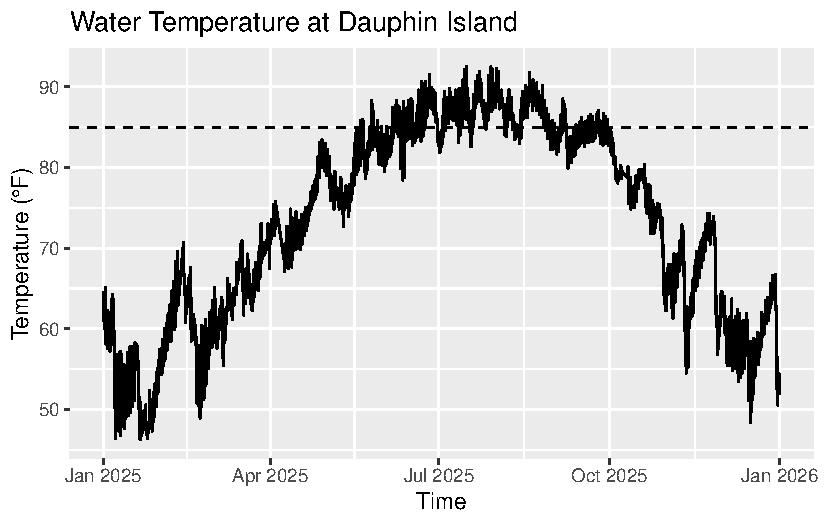
\includegraphics[keepaspectratio]{draft-results_files/figure-pdf/unnamed-chunk-3-1.pdf}}

\section{Secondary Analysis}\label{secondary-analysis-1}

The secondary analysis examines electricity demand patterns during
periods when water temperatures exceed 85°F.

Dates with water temperatures above 85°F were identified and overlaid on
the electricity demand time series. Red points in Figure 2 indicate days
when water temperatures exceeded the 85°F threshold.

\begin{Shaded}
\begin{Highlighting}[]
\NormalTok{high\_temp\_dates }\OtherTok{\textless{}{-}}\NormalTok{ temp\_clean }\SpecialCharTok{\%\textgreater{}\%}
  \FunctionTok{filter}\NormalTok{(temp\_f }\SpecialCharTok{\textgreater{}} \DecValTok{85}\NormalTok{) }\SpecialCharTok{\%\textgreater{}\%}
  \FunctionTok{mutate}\NormalTok{(}\AttributeTok{date =} \FunctionTok{as.Date}\NormalTok{(datetime)) }\SpecialCharTok{\%\textgreater{}\%}
  \FunctionTok{distinct}\NormalTok{(date)}

\NormalTok{daily\_demand }\OtherTok{\textless{}{-}}\NormalTok{ demand\_clean }\SpecialCharTok{\%\textgreater{}\%}
  \FunctionTok{mutate}\NormalTok{(}\AttributeTok{date =} \FunctionTok{as.Date}\NormalTok{(datetime)) }\SpecialCharTok{\%\textgreater{}\%}
  \FunctionTok{group\_by}\NormalTok{(date) }\SpecialCharTok{\%\textgreater{}\%}
  \FunctionTok{summarize}\NormalTok{(}\AttributeTok{daily\_demand\_mw =} \FunctionTok{mean}\NormalTok{(demand\_mw, }\AttributeTok{na.rm =} \ConstantTok{TRUE}\NormalTok{))}

\FunctionTok{ggplot}\NormalTok{(daily\_demand, }\FunctionTok{aes}\NormalTok{(date, daily\_demand\_mw)) }\SpecialCharTok{+}
  \FunctionTok{geom\_line}\NormalTok{(}\AttributeTok{color =} \StringTok{"blue"}\NormalTok{) }\SpecialCharTok{+}
  \FunctionTok{geom\_point}\NormalTok{(}\AttributeTok{data =}\NormalTok{ daily\_demand }\SpecialCharTok{\%\textgreater{}\%} \FunctionTok{filter}\NormalTok{(date }\SpecialCharTok{\%in\%}\NormalTok{ high\_temp\_dates}\SpecialCharTok{$}\NormalTok{date),}
             \FunctionTok{aes}\NormalTok{(date, daily\_demand\_mw), }\AttributeTok{color =} \StringTok{"red"}\NormalTok{, }\AttributeTok{size =} \FloatTok{1.5}\NormalTok{) }\SpecialCharTok{+}
  \FunctionTok{labs}\NormalTok{(}
    \AttributeTok{title =} \StringTok{"Daily Electricity Demand with High Water Temperature Days Highlighted"}\NormalTok{,}
    \AttributeTok{x =} \StringTok{"Date"}\NormalTok{,}
    \AttributeTok{y =} \StringTok{"Demand (MW)"}
\NormalTok{  )}
\end{Highlighting}
\end{Shaded}

\pandocbounded{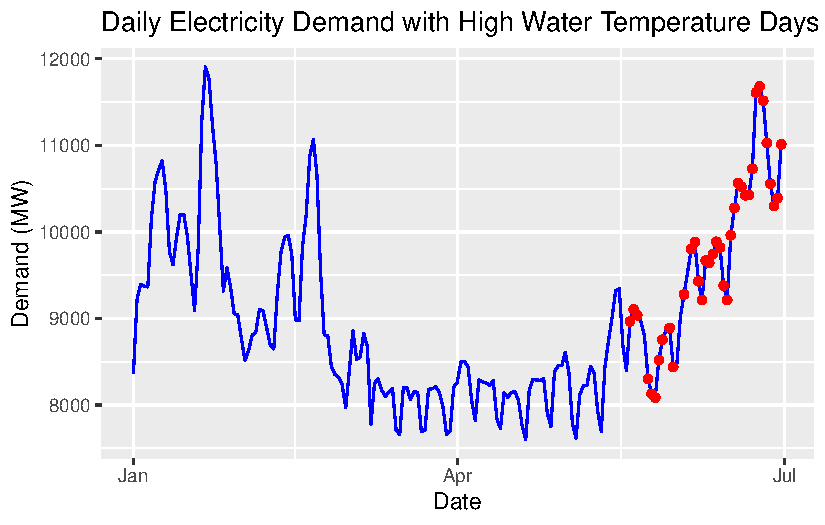
\includegraphics[keepaspectratio]{draft-results_files/figure-pdf/unnamed-chunk-4-1.pdf}}

High water temperature days occur primarily during the summer portion of
the electricity demand curve. Figure 2 shows that many of these days
coincide with periods of higher electricity demand, but interestingly
show these days also occur during local minimums.

\begin{tcolorbox}[enhanced jigsaw, rightrule=.15mm, breakable, opacitybacktitle=0.6, opacityback=0, colframe=quarto-callout-note-color-frame, toprule=.15mm, leftrule=.75mm, colbacktitle=quarto-callout-note-color!10!white, bottomrule=.15mm, arc=.35mm, bottomtitle=1mm, left=2mm, toptitle=1mm, titlerule=0mm, colback=white, coltitle=black, title=\textcolor{quarto-callout-note-color}{\faInfo}\hspace{0.5em}{Note}]

You might want to generate both pictures and line them up (facet by
variable, so that you have two rows), with some red highlighting behind
the temperature line (a rectangle with ymin = -Inf and ymax = Inf,
fill=``red'', alpha=0.1 or so), where the highlighting then extends to
the demand plot. That would make it easier to see a relationship.

\end{tcolorbox}

\section{Note to add second half of 2025
later}\label{note-to-add-second-half-of-2025-later}

\begin{tcolorbox}[enhanced jigsaw, rightrule=.15mm, breakable, opacitybacktitle=0.6, opacityback=0, colframe=quarto-callout-note-color-frame, toprule=.15mm, leftrule=.75mm, colbacktitle=quarto-callout-note-color!10!white, bottomrule=.15mm, arc=.35mm, bottomtitle=1mm, left=2mm, toptitle=1mm, titlerule=0mm, colback=white, coltitle=black, title=\textcolor{quarto-callout-note-color}{\faInfo}\hspace{0.5em}{Note}]

Make sure you're finishing your results section by evaluating what the
results mean in the context of the problem.

\end{tcolorbox}

\chapter{Draft: Intro/Conclusions}\label{draft-introconclusions}

\chapter{Introduction}\label{introduction-1}

Electric power systems are very sensitive to environmental conditions,
particularly temperature. Power plants that rely on nearby water bodies
as heat sinks may have operational constraints when water temperatures
rise above certain thresholds. As climate change continues, the risk of
higher water temperatures becomes a concern.

Previous research and data show that water temperature varies seasonally
and can become quite high during summer, particularly in regions such as
the Gulf of Mexico. {[}citation needed{]} In addition, electricity
demand tends to increase during the summer due to increased cooling
needs. {[}citation needed{]} This overlap creates potential stress on
power systems when both supply constraints and demand pressures happen
simultaneously.

This study aims to assess the risk that a coastal power plant near
Dauphin Island, Alabama will need to operate at reduced capacity.
Specifically, it looks at the frequency and timing of high water
temperature and compares these periods with patterns in regional
electricity demand.

To address this question, data from the National Oceanic and Atmospheric
Administration (NOAA) and the U.S. Energy Information Administration
(EIA) are analyzed {[}how?{]} to evaluate temperature and demand trends.

\chapter{Conclusion}\label{conclusion-1}

This analysis evaluated the risk that a coastal power plant near Dauphin
Island, Alabama, will be forced to operate at reduced capacity due to
elevated water temperatures. The results show that water temperatures
exceeding 85°F occur primarily during summer months.

These high temperature periods overlap with times of increased
electricity demand. This suggests that the plant may face increased
strain during critical times.

Overall, the findings indicate risk of reduced operating capacity within
the next five years. This risk is most clear during peak summer demand,
when system resilience is most important.

\begin{tcolorbox}[enhanced jigsaw, rightrule=.15mm, breakable, opacitybacktitle=0.6, opacityback=0, colframe=quarto-callout-note-color-frame, toprule=.15mm, leftrule=.75mm, colbacktitle=quarto-callout-note-color!10!white, bottomrule=.15mm, arc=.35mm, bottomtitle=1mm, left=2mm, toptitle=1mm, titlerule=0mm, colback=white, coltitle=black, title=\textcolor{quarto-callout-note-color}{\faInfo}\hspace{0.5em}{Note}]

Can you think of some possible solutions to investigate? e.g.~drawing
water from more depth (cooler) or improving thermal efficiency elsewhere
in the plant?

You need a bit more text here -- recap, weaknesses of the model,
limiting assumptions, and how does this report help an executive make
some decisions? Once you have more text, increase how skimmable this is
by putting some stuff in a box for an executive to focus on.

\end{tcolorbox}

\chapter{Draft: Executive Summary}\label{draft-executive-summary}

This report evaluates the risk that a coastal power plant near Dauphin
Island, Alabama will be forced to operate at reduced capacity due to
elevated gulf water temperatures. The plant relies on water from the
gulf as a heat sink and has to reduce output when temperatures exceed
85°F. The goal of this analysis is to see how often this threshold is
exceeded and whether these periods correlate with electricity demand.

Two publicly available datasets were analyzed in order to address this.
Water temperature data from NOAA was used to find periods when
temperatures exceed the threshold. Electricity demand data from the U.S.
Energy Information Administration (EIA) was used to examine when peak
demand occurs. These datasets were cleaned, aligned, and summarized
using graphically and descriptively.

The results show that water temperatures above 85°F occur often during
summer months. These periods overlap with increases in electricity
demand, which are likely driven by cooling needs. This creates a
situation where the plant may have to reduce output at the same time
demand is highest.

\textbf{Conclusion:} The plant faces a strong risk of reduced operating
capacity during high demand periods, especially in the summer. This
overlap increases the likelihood of strain on the electrical system and
reduces flexibility.

\textbf{Recommendations:} - Evaluate possible other cooling strategies
to reduce dependence on the gulf - Incorporate temperature risk into
planning for future operations

Overall, this analysis indicates that rising water temperatures are a
risk that should be accounted for in future planning and
decision-making.




\end{document}
